\chapter{The reusable core}
\label{ch:second}

For the sup norm $\norm{v}_\infty=\max_s\abs{v(s)}$ the operator is a $\gamma$-contraction:
\[
 \norm{\mathcal{T}^{\pi}v-\mathcal{T}^{\pi}w}_\infty\leq\gamma\norm{v-w}_\infty.
\]

\section{A figure with an e-reader twin}

Print gets TikZ; the EPUB and Markdown editions get the SVG inside \texttt{epubonly}.

\begin{center}
\begin{tikzpicture}[scale=0.9,>=Latex]
  \draw[->,gray!65] (-0.2,0) -- (5.0,0) node[right] {$x_1$};
  \draw[->,gray!65] (0,-0.2) -- (0,3.7) node[above] {$x_2$};
  \draw[->,very thick,teal] (0,0) -- (4,1) node[below right] {$u$};
  \draw[->,very thick,navy] (0,0) -- (2.3,3) node[above] {$x$};
  \draw[->,very thick,gold] (0,0) -- (2.87,0.72) node[below right] {$\operatorname{proj}_u(x)$};
  \draw[dashed,gold] (2.3,3) -- (2.87,0.72);
\end{tikzpicture}
\end{center}

\begin{epubonly}
\begin{figure}
\centering
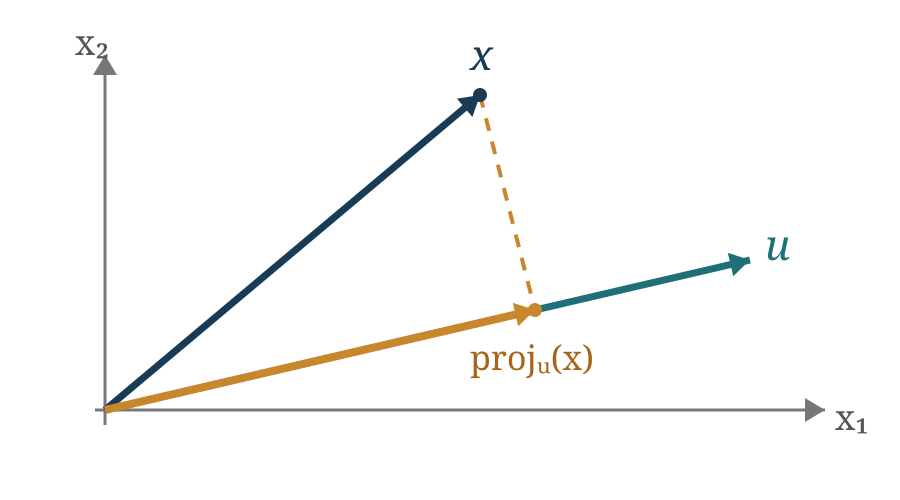
\includegraphics[alt={Vector x projected onto direction u, leaving an orthogonal residual.}]{epub/assets/projection.svg}
\caption{Projection keeps the component parallel to the chosen direction.}
\end{figure}
\end{epubonly}

\intuition{Projection keeps the part a representation can express and discards an
orthogonal residual.}

\practice{
\textbf{2.1} Prove $\abs{\max_a x_a-\max_a y_a}\leq\max_a\abs{x_a-y_a}$.
}
